% F092｜高中数学常用数值表｜05_traps.tex
% 继承上传模板的 LaTeX 环境；当前条目的内容独立编写。
\clearpage
\begin{trapbox}
\textbf{\textcolor{CTrap}{易错一：把截断写成四舍五入}}
\par\medskip
\begin{center}
% F092｜round 原创简明教学示意图
\begin{tikzpicture}[>=stealth,scale=.9]
\node[draw,rounded corners,fill=orange!10,minimum width=4cm,minimum height=1.1cm] (a) at (0,0){$\ln10=2.302585\ldots$};
\node[draw,rounded corners,fill=teal!12,minimum width=3.5cm,minimum height=1.1cm] (b) at (5.7,0){$\approx2.303$};
\draw[->,thick] (a)--node[above]{\small 保留三位}(b);
\node at (3,-1.1){\small 不要把已经舍入的数字再当成精确值};
\end{tikzpicture}

\end{center}
\medskip
$\ln10=2.302585\ldots$，保留三位小数是 $\boxed{2.303}$，而不是 $2.302$。原PDF中由 $0.693+1.609$ 得到 $2.302$ 是\textbf{近似值相加}，不可替代真值舍入。
\end{trapbox}
\clearpage
\begin{trapbox}
\textbf{\textcolor{CTrap}{易错二：多次使用已取三位小数的数字}}
\par\medskip
\begin{center}
% F092｜derive 原创简明教学示意图
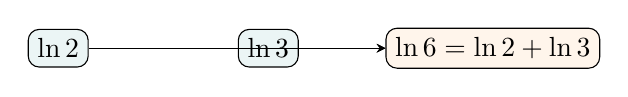
\begin{tikzpicture}[>=stealth,scale=.92]
\node[draw,rounded corners,fill=teal!8] (a) at (0,0){$\ln2$};
\node[draw,rounded corners,fill=teal!8] (b) at (2.9,0){$\ln3$};
\node[draw,rounded corners,fill=orange!8] (c) at (6,0){$\ln6=\ln2+\ln3$};
\draw[->] (a)--(c);\draw[->] (b)--(c);
\end{tikzpicture}

\end{center}
\medskip
$\ln9=2\ln3\approx2\times1.099=2.198$，但实际 $\ln9\approx2.197$（三位小数）。原因是 $\ln3\approx1.098612\ldots$，提前保留三位会损失末位。
\end{trapbox}
\clearpage
\begin{trapbox}
\textbf{\textcolor{CTrap}{易错三：把记忆表当证明}}
\par\medskip
\begin{center}
% F092｜square 原创简明教学示意图
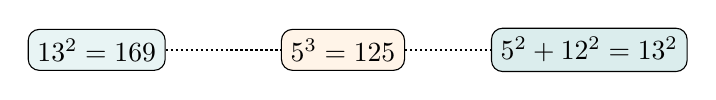
\begin{tikzpicture}[>=stealth,scale=.92]
\node[draw,rounded corners,fill=teal!9] (a) at (0,0){$13^2=169$};
\node[draw,rounded corners,fill=orange!9] (b) at (3.4,0){$5^3=125$};
\node[draw,rounded corners,fill=teal!14] (c) at (6.8,0){$5^2+12^2=13^2$};
\draw[densely dotted,thick] (a)--(b);\draw[densely dotted,thick] (b)--(c);
\end{tikzpicture}

\end{center}
\medskip
背熟 $3,4,5$ 有利于提速，但若题目要求证明一组数是勾股数组，仍需验 $a^2+b^2=c^2$。表中数据只有在适用条件下才能直接用。
\end{trapbox}
